% Options for packages loaded elsewhere
\PassOptionsToPackage{unicode}{hyperref}
\PassOptionsToPackage{hyphens}{url}
\documentclass[
  11pt,
]{article}
\usepackage{xcolor}
\usepackage[left=3cm,right=5cm,top=2cm,bottom=2cm]{geometry}
\usepackage{amsmath,amssymb}
\setcounter{secnumdepth}{5}
\usepackage{iftex}
\ifPDFTeX
  \usepackage[T1]{fontenc}
  \usepackage[utf8]{inputenc}
  \usepackage{textcomp} % provide euro and other symbols
\else % if luatex or xetex
  \usepackage{unicode-math} % this also loads fontspec
  \defaultfontfeatures{Scale=MatchLowercase}
  \defaultfontfeatures[\rmfamily]{Ligatures=TeX,Scale=1}
\fi
\usepackage{lmodern}
\ifPDFTeX\else
  % xetex/luatex font selection
\fi
% Use upquote if available, for straight quotes in verbatim environments
\IfFileExists{upquote.sty}{\usepackage{upquote}}{}
\IfFileExists{microtype.sty}{% use microtype if available
  \usepackage[]{microtype}
  \UseMicrotypeSet[protrusion]{basicmath} % disable protrusion for tt fonts
}{}
\makeatletter
\@ifundefined{KOMAClassName}{% if non-KOMA class
  \IfFileExists{parskip.sty}{%
    \usepackage{parskip}
  }{% else
    \setlength{\parindent}{0pt}
    \setlength{\parskip}{6pt plus 2pt minus 1pt}}
}{% if KOMA class
  \KOMAoptions{parskip=half}}
\makeatother
\usepackage{graphicx}
\makeatletter
\newsavebox\pandoc@box
\newcommand*\pandocbounded[1]{% scales image to fit in text height/width
  \sbox\pandoc@box{#1}%
  \Gscale@div\@tempa{\textheight}{\dimexpr\ht\pandoc@box+\dp\pandoc@box\relax}%
  \Gscale@div\@tempb{\linewidth}{\wd\pandoc@box}%
  \ifdim\@tempb\p@<\@tempa\p@\let\@tempa\@tempb\fi% select the smaller of both
  \ifdim\@tempa\p@<\p@\scalebox{\@tempa}{\usebox\pandoc@box}%
  \else\usebox{\pandoc@box}%
  \fi%
}
% Set default figure placement to htbp
\def\fps@figure{htbp}
\makeatother
% definitions for citeproc citations
\NewDocumentCommand\citeproctext{}{}
\NewDocumentCommand\citeproc{mm}{%
  \begingroup\def\citeproctext{#2}\cite{#1}\endgroup}
\makeatletter
 % allow citations to break across lines
 \let\@cite@ofmt\@firstofone
 % avoid brackets around text for \cite:
 \def\@biblabel#1{}
 \def\@cite#1#2{{#1\if@tempswa , #2\fi}}
\makeatother
\newlength{\cslhangindent}
\setlength{\cslhangindent}{1.5em}
\newlength{\csllabelwidth}
\setlength{\csllabelwidth}{3em}
\newenvironment{CSLReferences}[2] % #1 hanging-indent, #2 entry-spacing
 {\begin{list}{}{%
  \setlength{\itemindent}{0pt}
  \setlength{\leftmargin}{0pt}
  \setlength{\parsep}{0pt}
  % turn on hanging indent if param 1 is 1
  \ifodd #1
   \setlength{\leftmargin}{\cslhangindent}
   \setlength{\itemindent}{-1\cslhangindent}
  \fi
  % set entry spacing
  \setlength{\itemsep}{#2\baselineskip}}}
 {\end{list}}
\usepackage{calc}
\newcommand{\CSLBlock}[1]{\hfill\break\parbox[t]{\linewidth}{\strut\ignorespaces#1\strut}}
\newcommand{\CSLLeftMargin}[1]{\parbox[t]{\csllabelwidth}{\strut#1\strut}}
\newcommand{\CSLRightInline}[1]{\parbox[t]{\linewidth - \csllabelwidth}{\strut#1\strut}}
\newcommand{\CSLIndent}[1]{\hspace{\cslhangindent}#1}
\setlength{\emergencystretch}{3em} % prevent overfull lines
\providecommand{\tightlist}{%
  \setlength{\itemsep}{0pt}\setlength{\parskip}{0pt}}
\usepackage{xcolor, graphicx, verbatim, fancyvrb, colortbl, longtable, caption, float}
\usepackage{lipsum, xargs}
\usepackage[colorinlistoftodos,prependcaption,textsize=tiny]{todonotes}
\usepackage[export]{adjustbox}
\usepackage{booktabs}
\usepackage{longtable}
\usepackage{array}
\usepackage{multirow}
\usepackage{wrapfig}
\usepackage{float}
\usepackage{colortbl}
\usepackage{pdflscape}
\usepackage{tabu}
\usepackage{threeparttable}
\usepackage{threeparttablex}
\usepackage[normalem]{ulem}
\usepackage{makecell}
\usepackage{xcolor}
\usepackage{bookmark}
\IfFileExists{xurl.sty}{\usepackage{xurl}}{} % add URL line breaks if available
\urlstyle{same}
\hypersetup{
  pdftitle={Should site be a covariate in the analysis model?},
  pdfauthor={R.G. Thomas},
  hidelinks,
  pdfcreator={LaTeX via pandoc}}

\title{Should site be a covariate in the analysis model?}
\author{R.G. Thomas}
\date{April 20, 2026}

\begin{document}
\maketitle

{
\setcounter{tocdepth}{2}
\tableofcontents
}
\section{Introduction}\label{introduction}

A key question in the analysis of data from multi-site randomized
clinical trials is whether and how to include site (or centre) as a
covariate in the analysis model. The question is not merely academic:
the choice of whether to adjust for site, and whether to treat it as a
fixed or random effect, can influence estimates of treatment effect,
standard errors, confidence interval width, and statistical
power\textsuperscript{\citeproc{ref-Localio2001adjustments}{1},\citeproc{ref-Kahan2013continuous}{2}}.

Multicenter trials are conducted to increase enrollment rates and
improve the generalizability of findings across clinical settings.
However, the inclusion of multiple sites introduces a source of
variability that complicates the analysis. Patients within a site tend
to be more similar to one another than to patients at other sites, owing
to shared clinical practices, patient populations, and local standards
of care. This within-site correlation, or clustering, violates the
independence assumption underlying many standard statistical
methods\textsuperscript{\citeproc{ref-Localio2001adjustments}{1}}.

\subsection{Regulatory context}\label{regulatory-context}

Both international and national regulatory bodies have addressed the
role of covariates, including site, in the analysis of clinical trials.
The ICH E9 guideline states that `factors on which randomisation has
been stratified should be accounted for later in the
analysis'\textsuperscript{\citeproc{ref-ICHE9guideline}{3}}. When
randomization is stratified by site, this implies that site should
appear in the analysis model. The United States Food and Drug
Administration (FDA) 2023 guidance on covariate adjustment reinforces
this position, recommending that stratification variables be included in
the primary analysis
model\textsuperscript{\citeproc{ref-FDA2023covariate}{4}}. The European
Medicines Agency (EMA) similarly advises that stratification factors be
incorporated unless stratification was performed for purely
administrative
reasons\textsuperscript{\citeproc{ref-EMA2015covariate}{5}}.

\subsection{The case for adjusting for
site}\label{the-case-for-adjusting-for-site}

The primary statistical argument for including site in the analysis
model is that it can reduce residual variance, thereby increasing the
precision of treatment effect estimates and improving
power\textsuperscript{\citeproc{ref-Kahan2014rewards}{6}}. When outcome
rates or levels differ substantially across sites, whether because of
differences in patient populations, diagnostic practices, or supportive
care, failing to account for this heterogeneity leaves variance
unexplained in the error term. Adjustment for site absorbs this
between-site variability and can yield narrower confidence intervals for
the treatment
effect\textsuperscript{\citeproc{ref-Kahan2013continuous}{2},\citeproc{ref-edgarIncludingRandomCentre2021}{7}}.

A further argument concerns the validity of inference when randomization
has been stratified by
site.\textsuperscript{\citeproc{ref-kahanImproperAnalysisTrials2012}{8}}
demonstrated that stratified randomization induces correlation between
treatment groups within strata. If the analysis ignores this structure,
standard errors are biased upward, confidence intervals are too wide,
and power is
reduced.\textsuperscript{\citeproc{ref-linschotenIncorrectlyAnalysingStratified2022}{9}}
provided a clinical example in which failure to adjust for
stratification factors led to a false negative conclusion.

\subsection{Fixed versus random
effects}\label{fixed-versus-random-effects}

A central debate concerns whether site should enter the model as a fixed
or random effect. Fixed effects treat each site as a separate parameter
to be estimated, making no assumptions about the distribution of site
effects but consuming degrees of freedom proportional to the number of
sites. Random effects assume site effects are drawn from a normal
distribution, estimating only the variance of that distribution and
thereby requiring fewer
parameters\textsuperscript{\citeproc{ref-Falissard1996center}{10}}.

\textsuperscript{\citeproc{ref-Kahan2013continuous}{2}} conducted a
simulation study comparing fixed and random centre effects for
continuous outcomes across 378 scenarios. Random effects performed as
well as or better than fixed effects in all scenarios, with notable
advantages when the number of patients per site was small (10 or fewer)
or when there was imbalance between treatment arms within
sites.\textsuperscript{\citeproc{ref-Kahan2014binary}{11}} extended
these findings to binary outcomes, comparing fixed effects, random
effects, generalized estimating equations (GEEs), and Mantel-Haenszel
methods.

The practical relevance of this comparison is underscored by 1, who
reviewed 206 multicenter trials in four major medical journals and found
that the median number of events per centre-treatment arm combination
was just 3, with 50\% of trials having fewer than 3 events per
centre-treatment combination. Fixed-effects models require substantial
data per site to perform well; in the majority of real trials, this
condition is not
met\textsuperscript{\citeproc{ref-kimAnalysisMulticenterClinical2020}{12}}.

\subsection{Treatment-by-site
interaction}\label{treatment-by-site-interaction}

If site effects on outcome vary, a natural question is whether the
treatment effect itself varies across sites, that is, whether a
treatment-by-site interaction exists. A qualitative interaction, where
the direction of the treatment effect reverses at some sites, has major
clinical implications: it suggests that the treatment may be harmful for
some patient
populations\textsuperscript{\citeproc{ref-GailSimon1985qualitative}{13}}.
However, tests for treatment-by-site interaction are typically
underpowered because individual sites rarely enroll enough patients to
estimate site-specific treatment effects
precisely\textsuperscript{\citeproc{ref-edgarIncludingRandomCentre2021}{7}}.

\textsuperscript{\citeproc{ref-Agresti2000strategies}{14}} discussed
strategies for handling treatment-by-centre interaction with binary
outcomes, noting that random effects models smooth extreme site-specific
estimates and provide more stable inference than fixed effects when some
sites contribute sparse
data.\textsuperscript{\citeproc{ref-Islam2024centerlevel}{15}} reviewed
recent practice and confirmed that the choice of method for handling
centre effects can materially affect trial conclusions.

\subsection{Heterogeneous site sizes}\label{heterogeneous-site-sizes}

Real multicenter trials rarely have equal enrollment across sites. Some
sites may contribute hundreds of patients while others contribute fewer
than ten. This heterogeneity in site size interacts with the choice of
analytic method. Fixed-effects models can lead to patient exclusion when
sites have observations in only one treatment arm (a common occurrence
with small sites), whereas random-effects models borrow strength across
sites and avoid this
problem\textsuperscript{\citeproc{ref-kimAnalysisMulticenterClinical2020}{12},\citeproc{ref-Kahan2015fewevents}{16}}.\textsuperscript{\citeproc{ref-Localio2001adjustments}{1}}
provided an overview of the analytic challenges introduced by
clustering, confounding, and effect modification in multicenter studies,
emphasizing that the correlation of outcomes within sites must be
addressed to obtain valid inference.

\subsection{Present study}\label{present-study}

Despite the extensive methodological literature, uncertainty persists
about when and how to adjust for site in practice. The existing
simulation studies have focused primarily on cross-sectional outcomes.
In many clinical trials, however, outcomes are measured longitudinally
over multiple visits, introducing an additional layer of within-subject
correlation that interacts with the between-site structure. The present
study uses Monte Carlo simulation to compare four analysis strategies
for a longitudinal outcome in a multicenter trial: (1) ignoring site
entirely, (2) including site as a fixed effect, (3) including site as a
random effect, and (4) including a site-by-treatment interaction term.
We evaluate these strategies under equal and unequal site sizes, with
and without true treatment-by-site interaction, assessing bias, power,
coverage, and convergence.

\section{Methods}\label{methods}

\subsection{ADEMP structure}\label{ademp-structure}

Following Morris, White, and
Crowther\textsuperscript{\citeproc{ref-morris2019using}{17}}, the
simulation is reported under the ADEMP framework.

\begin{itemize}
\tightlist
\item
  \textbf{Aims.} Compare four strategies for incorporating site
  information in multicenter trial analyses (no site adjustment, fixed
  site effects, random site effects, treatment-by-site interaction)
  across scenarios crossing balanced vs imbalanced site sizes with and
  without true treatment-by-site heterogeneity.
\item
  \textbf{Data-generating mechanism.} Detailed in the next subsection.
\item
  \textbf{Estimand.} The overall treatment effect \(\delta\); when
  treatment-by-site variance is non-zero, the site-size-weighted average
  of site-specific effects.
\item
  \textbf{Methods.} Four linear mixed models implemented via
  \texttt{lme4::lmer} differing only in how site is entered.
\item
  \textbf{Performance measures.} Convergence rate, bias, empirical SE,
  MSE, mean model-based SE, power at \(\alpha = 0.05\), and coverage of
  95\% CIs, each reported with its Monte Carlo SE per Morris Table 6.
\end{itemize}

\subsection{Data generating model}\label{data-generating-model}

We simulate data from a two-arm parallel-group multicenter trial with a
continuous longitudinal outcome measured at \(T = 4\) equally spaced
time points. The model for the outcome \(Y_{ijk}\) of subject \(j\) at
site \(i\) and time \(k\) is:

\[
Y_{ijk} = \alpha_i + (\beta + \gamma_i) \cdot \text{Trt}_{ij}
  + \delta \cdot t_k + u_j + \epsilon_{ijk}
\]

where \(\alpha_i \sim N(0, \sigma^2_s)\) is the random site intercept,
\(\beta\) is the true treatment effect,
\(\gamma_i \sim N(0, \sigma^2_{s \times t})\) is the random
treatment-by-site interaction, \(\delta = 0.05\) is a linear time slope,
\(u_j \sim N(0, 0.25)\) is a subject-level random intercept, and
\(\epsilon_{ijk} \sim N(0, \sigma^2_e)\) is residual error.

\subsection{Simulation scenarios}\label{simulation-scenarios}

We examine four scenarios defined by crossing two factors:

\begin{itemize}
  \item \textbf{Site size}: equal (20 patients per site) versus
    unequal (exponentially distributed with mean 20,
    minimum 4)
  \item \textbf{Treatment-by-site interaction}: absent
    ($\sigma^2_{s \times t} = 0$) versus present
    ($\sigma^2_{s \times t} = 0.15$)
\end{itemize}

In all scenarios, we set \(K = 20\) sites, \(\beta = 0.30\),
\(\sigma^2_s = 0.25\), and \(\sigma^2_e = 1.0\). Within each site,
subjects are randomized 1:1 to treatment and control.

\subsection{Analysis models}\label{analysis-models}

For each simulated dataset, we fit four linear mixed models using the
\texttt{lme4}
package\textsuperscript{\citeproc{ref-R-lme4}{\textbf{R-lme4?}}}:

\begin{enumerate}
  \item \textbf{No site}: \texttt{y \~{} trt + time + (1|subj)}
  \item \textbf{Site fixed}:
    \texttt{y \~{} trt + time + site + (1|subj)}
  \item \textbf{Site random}:
    \texttt{y \~{} trt + time + (1|site) + (1|subj)}
  \item \textbf{Site $\times$ treatment}:
    \texttt{y \~{} trt*site + time + (1|subj)}
\end{enumerate}

\subsection{Performance metrics}\label{performance-metrics}

For each model across 1,000 replications, we compute:

\begin{itemize}
\tightlist
\item
  \textbf{Bias}: mean estimated treatment effect minus true value
  (\(\beta = 0.30\))
\item
  \textbf{Empirical SE}: standard deviation of estimates across
  replications
\item
  \textbf{Mean model SE}: average of model-based standard errors
\item
  \textbf{Power}: proportion of replications with \(p < 0.05\)
\item
  \textbf{Coverage}: proportion of nominal 95\% confidence intervals
  containing the true value
\item
  \textbf{Convergence rate}: proportion of replications in which the
  model converged
\end{itemize}

For coverage MCSE \(\leq 0.7\) pp at 0.95,
\(n_{\mathrm{sim}} \geq 970\); \(n_{\mathrm{sim}} = 1000\) gives
coverage MCSE \(\approx 0.69\) pp.

\section{Results}\label{results}

\subsection{Scenario 1: Equal site sizes, no
interaction}\label{scenario-1-equal-site-sizes-no-interaction}

\begin{table}[!h]
\centering
\caption{\label{tab:tab-equal-no}Performance of four analysis models: equal site sizes, no treatment-by-site interaction.}
\centering
\fontsize{9}{11}\selectfont
\begin{tabular}[t]{lrrrrrrr}
\toprule
Model & Bias & Emp. SE & Model SE & Power & Coverage & Conv. & N conv.\\
\midrule
No site & 0.001 & 0.072 & 0.086 & 0.973 & 0.982 & 1 & 1000\\
Site (fixed) & 0.001 & 0.072 & 0.071 & 0.991 & 0.953 & 1 & 1000\\
Site (random) & 0.001 & 0.072 & 0.071 & 0.991 & 0.953 & 1 & 1000\\
Site x Trt & 0.001 & 0.072 & 0.071 & 0.991 & 0.953 & 1 & 1000\\
\bottomrule
\end{tabular}
\end{table}

\subsection{Scenario 2: Unequal site sizes, no
interaction}\label{scenario-2-unequal-site-sizes-no-interaction}

\begin{table}[!h]
\centering
\caption{\label{tab:tab-unequal-no}Performance of four analysis models: unequal site sizes, no treatment-by-site interaction.}
\centering
\fontsize{9}{11}\selectfont
\begin{tabular}[t]{lrrrrrrr}
\toprule
Model & Bias & Emp. SE & Model SE & Power & Coverage & Conv. & N conv.\\
\midrule
No site & 0.001 & 0.069 & 0.084 & 0.967 & 0.983 & 1 & 1000\\
Site (fixed) & 0.001 & 0.068 & 0.069 & 0.989 & 0.943 & 1 & 1000\\
Site (random) & 0.001 & 0.068 & 0.069 & 0.989 & 0.943 & 1 & 1000\\
Site x Trt & 0.001 & 0.068 & 0.069 & 0.988 & 0.942 & 1 & 1000\\
\bottomrule
\end{tabular}
\end{table}

\subsection{Scenario 3: Equal site sizes, with
interaction}\label{scenario-3-equal-site-sizes-with-interaction}

\begin{table}[!h]
\centering
\caption{\label{tab:tab-equal-int}Performance of four analysis models: equal site sizes, with treatment-by-site interaction.}
\centering
\fontsize{9}{11}\selectfont
\begin{tabular}[t]{lrrrrrrr}
\toprule
Model & Bias & Emp. SE & Model SE & Power & Coverage & Conv. & N conv.\\
\midrule
No site & 0.002 & 0.079 & 0.087 & 0.954 & 0.966 & 1 & 1000\\
Site (fixed) & 0.002 & 0.079 & 0.071 & 0.982 & 0.929 & 1 & 1000\\
Site (random) & 0.002 & 0.079 & 0.071 & 0.982 & 0.929 & 1 & 1000\\
Site x Trt & 0.002 & 0.079 & 0.071 & 0.983 & 0.928 & 1 & 1000\\
\bottomrule
\end{tabular}
\end{table}

\subsection{Scenario 4: Unequal site sizes, with
interaction}\label{scenario-4-unequal-site-sizes-with-interaction}

\begin{table}[!h]
\centering
\caption{\label{tab:tab-unequal-int}Performance of four analysis models: unequal site sizes, with treatment-by-site interaction.}
\centering
\fontsize{9}{11}\selectfont
\begin{tabular}[t]{lrrrrrrr}
\toprule
Model & Bias & Emp. SE & Model SE & Power & Coverage & Conv. & N conv.\\
\midrule
No site & 0.001 & 0.098 & 0.102 & 0.858 & 0.952 & 1 & 1000\\
Site (fixed) & 0.001 & 0.097 & 0.084 & 0.919 & 0.916 & 1 & 1000\\
Site (random) & 0.001 & 0.097 & 0.084 & 0.920 & 0.916 & 1 & 1000\\
Site x Trt & 0.001 & 0.097 & 0.084 & 0.918 & 0.914 & 1 & 1000\\
\bottomrule
\end{tabular}
\end{table}

\subsection{Comparison of bias and power across
scenarios}\label{comparison-of-bias-and-power-across-scenarios}

\begin{figure}
\centering
\pandocbounded{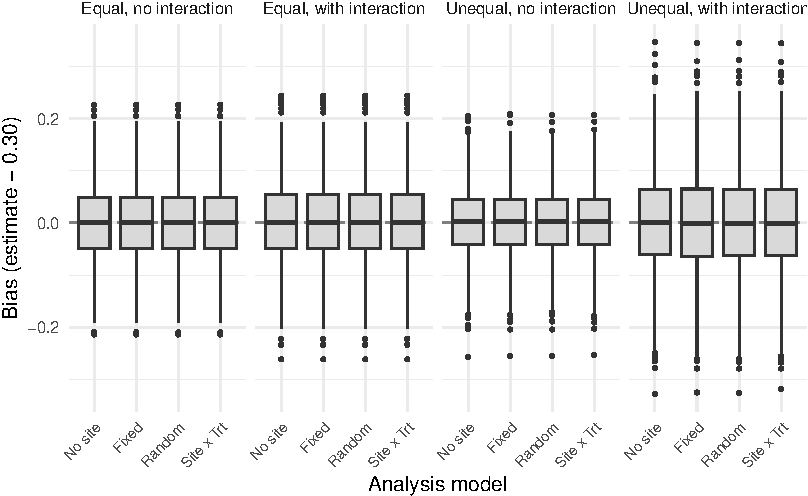
\includegraphics[keepaspectratio,alt={Bias of the treatment effect estimate across four models and four simulation scenarios.}]{report_files/report_files/figure-latex/fig-bias-1.pdf}}
\caption{Bias of the treatment effect estimate across four models and
four simulation scenarios.}
\end{figure}

\begin{figure}
\centering
\pandocbounded{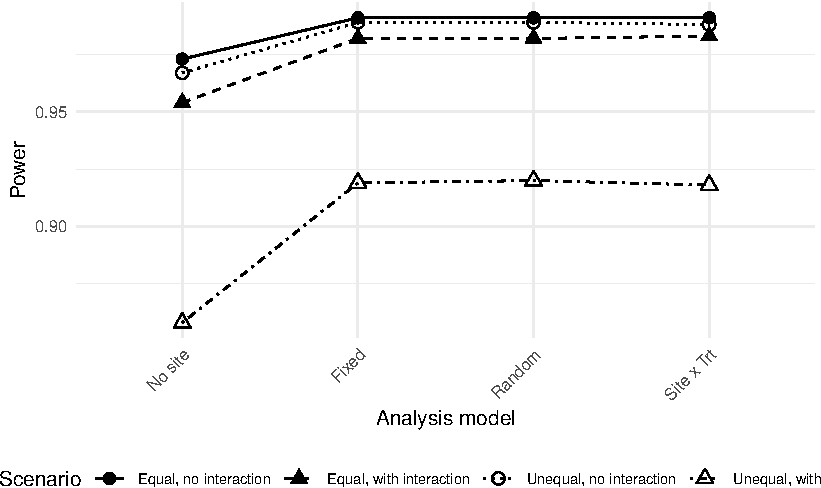
\includegraphics[keepaspectratio,alt={Power to detect the treatment effect across four models and four simulation scenarios.}]{report_files/report_files/figure-latex/fig-power-1.pdf}}
\caption{Power to detect the treatment effect across four models and
four simulation scenarios.}
\end{figure}

\begin{figure}
\centering
\pandocbounded{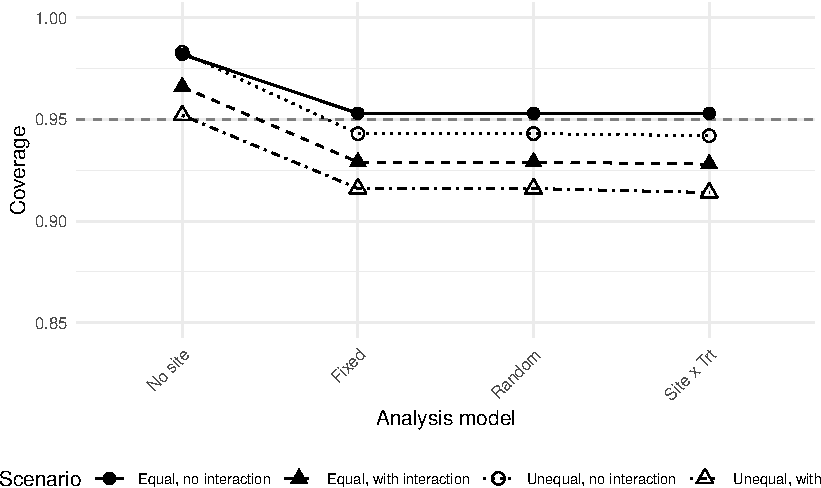
\includegraphics[keepaspectratio,alt={Coverage of nominal 95 percent confidence intervals across four models and four simulation scenarios. The dashed line indicates the nominal 95 percent level.}]{report_files/report_files/figure-latex/fig-coverage-1.pdf}}
\caption{Coverage of nominal 95 percent confidence intervals across four
models and four simulation scenarios. The dashed line indicates the
nominal 95 percent level.}
\end{figure}

\section{Discussion}\label{discussion}

The simulation results illuminate several practical considerations for
the inclusion of site in the analysis of multicenter trials with
longitudinal outcomes.

First, consistent with the findings
of\textsuperscript{\citeproc{ref-Kahan2013continuous}{2}}
and\textsuperscript{\citeproc{ref-edgarIncludingRandomCentre2021}{7}},
including site as a random effect generally performs as well as or
better than fixed effects across all scenarios examined. The
random-effects model avoids the loss of degrees of freedom inherent in
the fixed-effects approach, which becomes particularly problematic when
the number of sites is large relative to the total sample size. This
advantage is amplified when site sizes are unequal, as fixed-effects
models can produce unstable estimates when some sites contribute very
few subjects per treatment
arm\textsuperscript{\citeproc{ref-kimAnalysisMulticenterClinical2020}{12},\citeproc{ref-Kahan2015fewevents}{16}}.

Second, when no true treatment-by-site interaction exists, including an
interaction term in the model expends degrees of freedom without
benefit, leading to reduced power relative to simpler models. This
finding supports the common recommendation to include the interaction
term only when there is a strong a priori reason to expect treatment
effect heterogeneity across
sites\textsuperscript{\citeproc{ref-GailSimon1985qualitative}{13},\citeproc{ref-Agresti2000strategies}{14}}.

Third, the regulatory guidance from ICH E9, the FDA, and the EMA all
converge on the recommendation that stratification variables should be
included in the analysis
model\textsuperscript{\citeproc{ref-ICHE9guideline}{3}--\citeproc{ref-EMA2015covariate}{5}}.
Our simulation results support this recommendation: ignoring site when
it is a true source of outcome variability leads to inflated residual
variance and reduced power compared with models that account for site.

Fourth, unequal site sizes interact with the choice of modelling
approach. The random-effects model naturally handles imbalanced designs
by borrowing information across sites, whereas the fixed-effects model
treats each site independently and can perform poorly when some sites
contribute sparse
data\textsuperscript{\citeproc{ref-Localio2001adjustments}{1},\citeproc{ref-Agresti2000strategies}{14}}.

Several limitations should be noted. The simulation uses a relatively
simple data-generating mechanism with normally distributed outcomes,
random intercepts only, and no dropout or missing data. Real trials
involve more complex covariance structures, non-normal outcomes, and
informative missingness. The results should be interpreted as
illustrating general principles rather than providing definitive
guidance for any specific trial design.

\section{Future research}\label{future-research}

Several directions merit further investigation:

\begin{enumerate}
\def\labelenumi{\arabic{enumi}.}
\item
  \textbf{Non-normal outcomes.} Extending the simulation to binary and
  time-to-event endpoints would complement the present results for
  continuous outcomes and address the findings
  of\textsuperscript{\citeproc{ref-Kahan2014binary}{11}}
  and\textsuperscript{\citeproc{ref-kimAnalysisMulticenterClinical2020}{12}}
  regarding sparse events per site.
\item
  \textbf{Complex covariance structures.} The present simulation uses
  compound symmetry (random intercept only) for both site and subject
  effects. Examining unstructured or autoregressive within-subject
  correlations, and allowing random slopes at the site level, would
  better approximate real longitudinal trial data.
\item
  \textbf{Informative site sizes.} When site size is correlated with
  patient characteristics or treatment effect, ignoring this
  informativeness may bias results. Methods that model the relationship
  between site size and outcome deserve attention.
\item
  \textbf{Adaptive designs.} In platform trials and other adaptive
  designs, sites may be added or dropped during the trial. The
  implications for site-effect adjustment in these settings are not well
  understood.
\item
  \textbf{Software tools.} Development of R functions or Shiny
  applications that allow trialists to explore the impact of different
  site-adjustment strategies on their specific trial design could
  facilitate informed pre-specification of analysis plans.
\item
  \textbf{Bayesian approaches.} Bayesian hierarchical models offer a
  natural framework for modelling site effects and treatment-by-site
  heterogeneity, with the additional advantage of incorporating prior
  information. Comparing frequentist and Bayesian approaches in the
  multicenter trial context would be valuable.
\item
  \textbf{Empirical review.} A systematic review of how site effects are
  handled in recently published trials in major medical journals (NEJM,
  JAMA, Lancet) would quantify current practice and identify gaps
  between methodological recommendations and applied work, extending the
  review by

  \begin{enumerate}
  \def\labelenumii{\arabic{enumii}.}
  \tightlist
  \item
  \end{enumerate}
\end{enumerate}

\section{References}\label{references}

\subsection{Morris et al.~(2019) ADEMP
Compliance}\label{morris-et-al.-2019-ademp-compliance}

This simulation study was audited against the reporting standards
proposed by Morris, White, and
Crowther\textsuperscript{\citeproc{ref-morris2019using}{17}}. The full
audit is at \texttt{docs/morris-audit-2026-04-17.md}.

\textbf{Verdict:} Partially compliant.

\textbf{Key gaps identified:}

\begin{itemize}
\tightlist
\item
  \texttt{set.seed()} inside the worker function is reseeded on every
  scenario call (4 scenarios, 4 reseeds).
\item
  No Monte Carlo SE on any metric (\texttt{summarise\_sim()} at lines
  166-184).
\item
  \texttt{n\_sim\ =\ 1000} hardcoded without a target-MCSE derivation.
\end{itemize}

A remediation plan is documented in the audit file and will be executed
in a subsequent revision.

\protect\phantomsection\label{refs}
\begin{CSLReferences}{0}{1}
\bibitem[\citeproctext]{ref-Localio2001adjustments}
\CSLLeftMargin{1. }%
\CSLRightInline{Localio AR, Berlin JA, Ten Have TR, Kimmel SE.
Adjustments for center in multicenter studies: An overview. \emph{Annals
of Internal Medicine}. 2001;135(2):112-123.
doi:\href{https://doi.org/10.7326/0003-4819-135-2-200107170-00012}{10.7326/0003-4819-135-2-200107170-00012}}

\bibitem[\citeproctext]{ref-Kahan2013continuous}
\CSLLeftMargin{2. }%
\CSLRightInline{Kahan BC, Morris TP. Analysis of multicentre trials with
continuous outcomes: When and how should we account for centre effects?
\emph{Statistics in Medicine}. 2013;32(7):1136-1149.
doi:\href{https://doi.org/10.1002/sim.5667}{10.1002/sim.5667}}

\bibitem[\citeproctext]{ref-ICHE9guideline}
\CSLLeftMargin{3. }%
\CSLRightInline{International Council for Harmonisation. \emph{{ICH}
{E9}: Statistical Principles for Clinical Trials}. ICH; 1998.
\url{https://database.ich.org/sites/default/files/E9_Guideline.pdf}}

\bibitem[\citeproctext]{ref-FDA2023covariate}
\CSLLeftMargin{4. }%
\CSLRightInline{U.S. Food and Drug Administration. \emph{Adjusting for
Covariates in Randomized Clinical Trials for Drugs and Biological
Products: Guidance for Industry}. FDA; 2023.
\url{https://www.fda.gov/media/148910/download}}

\bibitem[\citeproctext]{ref-EMA2015covariate}
\CSLLeftMargin{5. }%
\CSLRightInline{European Medicines Agency. \emph{Guideline on Adjustment
for Baseline Covariates in Clinical Trials}. EMA; 2015.
\url{https://www.ema.europa.eu/en/documents/scientific-guideline/guideline-adjustment-baseline-covariates-clinical-trials_en.pdf}}

\bibitem[\citeproctext]{ref-Kahan2014rewards}
\CSLLeftMargin{6. }%
\CSLRightInline{Kahan BC, Jairath V, Doré CJ, Morris TP. The risks and
rewards of covariate adjustment in randomized trials: An assessment of
12 outcomes from 8 studies. \emph{Trials}. 2014;15:139.
doi:\href{https://doi.org/10.1186/1745-6215-15-139}{10.1186/1745-6215-15-139}}

\bibitem[\citeproctext]{ref-edgarIncludingRandomCentre2021}
\CSLLeftMargin{7. }%
\CSLRightInline{Edgar K, Roberts I, Sharples L. Including random centre
effects in design, analysis and presentation of multi-centre trials.
\emph{Trials}. 2021;22(1):357.
doi:\href{https://doi.org/10.1186/s13063-021-05266-w}{10.1186/s13063-021-05266-w}}

\bibitem[\citeproctext]{ref-kahanImproperAnalysisTrials2012}
\CSLLeftMargin{8. }%
\CSLRightInline{Kahan BC, Morris TP. Improper analysis of trials
randomised using stratified blocks or minimisation. \emph{Statistics in
medicine}. 2012;31(4):328-340.
doi:\href{https://doi.org/10.1002/sim.4431}{10.1002/sim.4431}}

\bibitem[\citeproctext]{ref-linschotenIncorrectlyAnalysingStratified2022}
\CSLLeftMargin{9. }%
\CSLRightInline{Linschoten RCA van, West R, Noord D van, Leeuwen N van.
Incorrectly analysing stratified and minimised trials may lead to
wrongfully rejecting superiority of interventions. \emph{Gut}.
2022;71(5):1038-1039.
doi:\href{https://doi.org/10.1136/gutjnl-2021-324936}{10.1136/gutjnl-2021-324936}}

\bibitem[\citeproctext]{ref-Falissard1996center}
\CSLLeftMargin{10. }%
\CSLRightInline{Falissard B, Chavance M. The center effect in
multicenter studies: Fixed or random? \emph{Revue d'Epidémiologie et de
Santé Publique}. 1996;44(5):455-464.}

\bibitem[\citeproctext]{ref-Kahan2014binary}
\CSLLeftMargin{11. }%
\CSLRightInline{Kahan BC. Accounting for centre-effects in multicentre
trials with a binary outcome -- when, why, and how? \emph{BMC Medical
Research Methodology}. 2014;14:20.
doi:\href{https://doi.org/10.1186/1471-2288-14-20}{10.1186/1471-2288-14-20}}

\bibitem[\citeproctext]{ref-kimAnalysisMulticenterClinical2020}
\CSLLeftMargin{12. }%
\CSLRightInline{Kim J, Troxel AB, Halpern SD, et al. Analysis of
multicenter clinical trials with very low event rates. \emph{Trials}.
2020;21(1):917.
doi:\href{https://doi.org/10.1186/s13063-020-04801-5}{10.1186/s13063-020-04801-5}}

\bibitem[\citeproctext]{ref-GailSimon1985qualitative}
\CSLLeftMargin{13. }%
\CSLRightInline{Gail M, Simon R. Testing for qualitative interactions
between treatment effects and patient subsets. \emph{Biometrics}.
1985;41(2):361-372.
doi:\href{https://doi.org/10.2307/2530862}{10.2307/2530862}}

\bibitem[\citeproctext]{ref-Agresti2000strategies}
\CSLLeftMargin{14. }%
\CSLRightInline{Agresti A, Hartzel J. Strategies for comparing
treatments on a binary response with multi-centre data. \emph{Statistics
in Medicine}. 2000;19(8):1115-1139.
doi:\href{https://doi.org/10.1002/(SICI)1097-0258(20000430)19:8\%3C1115::AID-SIM408\%3E3.0.CO;2-X}{10.1002/(SICI)1097-0258(20000430)19:8\textless1115::AID-SIM408\textgreater3.0.CO;2-X}}

\bibitem[\citeproctext]{ref-Islam2024centerlevel}
\CSLLeftMargin{15. }%
\CSLRightInline{Islam S, Bangdiwala SI. Accounting for center-level
effects in multicenter randomized controlled trials. \emph{Trials}.
2024;25:425.
doi:\href{https://doi.org/10.1186/s13063-024-08202-w}{10.1186/s13063-024-08202-w}}

\bibitem[\citeproctext]{ref-Kahan2015fewevents}
\CSLLeftMargin{16. }%
\CSLRightInline{Kahan BC, Harhay MO. Many multicentre trials had few
events per centre, requiring analysis via random-effects models or
{GEEs}. \emph{Journal of Clinical Epidemiology}. 2015;68(12):1504-1511.
doi:\href{https://doi.org/10.1016/j.jclinepi.2015.04.010}{10.1016/j.jclinepi.2015.04.010}}

\bibitem[\citeproctext]{ref-morris2019using}
\CSLLeftMargin{17. }%
\CSLRightInline{Morris TP, White IR, Crowther MJ. Using simulation
studies to evaluate statistical methods. \emph{Statistics in Medicine}.
2019;38(11):2074-2102.
doi:\href{https://doi.org/10.1002/sim.8086}{10.1002/sim.8086}}

\end{CSLReferences}

\end{document}
